\documentclass[11pt,a4paper]{article}

\usepackage[margin=2.4cm]{geometry}
\usepackage{booktabs}
\usepackage{siunitx}
\usepackage{amsmath}
\usepackage{xcolor}
\usepackage{pgfplots}
\usepackage{fancyvrb}
\usepackage{fvextra}
\usepackage[colorlinks=true,linkcolor=blue!55!black,urlcolor=blue!55!black]{hyperref}
\pgfplotsset{compat=1.16}
\sisetup{detect-weight=true}

\emergencystretch=3em
\hbadness=10000

\newcommand{\stdone}{{\color{green!55!black}\textbf{done}}}
\newcommand{\stpart}{{\color{orange!80!black}\textbf{partial}}}
\newcommand{\stopen}{{\color{red!70!black}\textbf{open}}}

\title{\textbf{SMARTSED --- GPU (CUDA) Port of the Deterministic Solver}\\[2pt]
\large Kernel port status, CPU-reference validation, and initial performance benchmark}
\author{Federico Gatti}
\date{\today}

\begin{document}
\maketitle

\begin{abstract}
\noindent
The deterministic SMARTSED solver (2D shallow-water / de Saint-Venant hydraulics
coupled to snow, infiltration, a gravitational sediment layer and Gavrilovi\'c
sediment production) has been ported to CUDA. The full inner time-stepping loop
now runs on the GPU: interface fluxes, friction, precipitation/infiltration,
\texttt{computeResiduals} (gravitational-layer fluxes), the snow / gravitational
layer update, bilinear velocity interpolation, the sediment-transport inner loop,
sparse-matrix assembly and the preconditioned CG solve (cuSPARSE/cuBLAS), plus
the water-height scatter, the velocity update and the adaptive time-step
reduction added in this iteration. The same source tree still compiles as a
pure-CPU reference (\texttt{-DENABLE\_CUDA=OFF}); a field-fingerprint harness
compares the two backends step by step. End-to-end GPU results track the CPU
reference to floating-point-reordering tolerance
($\sim\!5\times10^{-7}$ per step). An initial speed-up sweep over problem size
shows a crossover near $3\text{--}4\times10^{4}$ active cells: below it the
launch/-sync overhead makes the CPU faster, above it the GPU loop is
$\approx 2.2\text{--}2.3\times$ faster. The finest grid tested ($10$~m,
$2.7\times10^{5}$ cells) currently aborts in the CG solve and is the top
open item.
\end{abstract}

\section{Milestone status}

\begin{table}[h]
\centering
\small
\begin{tabular}{@{}p{0.50\linewidth}c p{0.34\linewidth}@{}}
\toprule
Deliverable & Status & Notes \\
\midrule
Working CUDA code (whole time loop on device)        & \stdone  & builds + runs, A40 \\
Port \texttt{computeResiduals}                        & \stdone  & \texttt{computeResiduals\{H,V\}\_wrapper} \\
Port \texttt{bilinearInterpolation}                   & \stdone  & \texttt{bilinearInterpolation\{H,V\}\_wrapper} \\
Port gravitational-layer update                       & \stdone  & \texttt{updateSnowGravLayers\_wrapper} \\
Port snow-accumulation loop                           & \stdone  & (same kernel) \\
Port sediment-transport inner loop                    & \stdone  & \texttt{computeResidualsTruncated-} \texttt{\{H,V\}\_wrapper} \\
Adaptive-$\Delta t$ reduction on device              & \stdone  & \texttt{thrust::transform\_reduce} \\
CPU reference from the same sources                   & \stdone  & \texttt{\#else} paths, this iteration \\
Full correctness validation vs.\ CPU                  & \stpart  & $H,\eta,u,v$ validated; sediment / snow layers inactive in the test event \\
Isolated per-kernel unit-test suite                  & \stopen  & only a system-level fingerprint harness so far \\
Per-kernel timing breakdown (NVTX / \texttt{cudaEvent}) & \stopen & only whole-loop wall-clock so far \\
Initial performance benchmark (speed-up table)        & \stdone  & Section~\ref{sec:bench} \\
$10$~m resolution on GPU                              & \stopen  & CG solve aborts, Section~\ref{sec:issues} \\
\bottomrule
\end{tabular}
\caption{Status against the milestone description.}
\end{table}

\section{Kernel port inventory}

\texttt{cuda\_utils\_loop\_H.cu} currently holds \textbf{38} \texttt{\_\_global\_\_}
kernels behind \textbf{17} host-side wrappers. Table~\ref{tab:kernels} maps each
physical stage of one time step to its wrapper(s).

\begin{table}[h]
\centering
\footnotesize
\setlength{\tabcolsep}{4pt}
\begin{tabular}{@{}p{0.38\linewidth}p{0.46\linewidth}c@{}}
\toprule
Stage of a time step & Wrapper(s) & Added \\
\midrule
Upwind interface heights $H_{x},H_{y}$      & \texttt{compute\_\{h,v\}\_interface\_wrapper} & earlier \\
$\alpha$ flux coefficients                  & (fused in interface / friction kernels) & earlier \\
Friction (Rickenmann / Manning)             & \texttt{compute\_\{h,v\}\_friction\_wrapper} & earlier \\
Temperature update                          & \texttt{computeTemperature\_wrapper} & earlier \\
Evapotranspiration                          & \texttt{computeET\_wrapper} & earlier \\
Precipitation / infiltration (SCS-CN)       & \texttt{computePrecipitation\_wrapper} & earlier \\
Gravitational-layer fluxes (\texttt{computeResiduals}) & \texttt{computeResiduals\{H,V\}\_wrapper} & earlier \\
Snow accumulation + gravitational layer     & \texttt{updateSnowGravLayers\_wrapper} & earlier \\
Bilinear interpolation $u^{*},v^{*}$        & \texttt{bilinearInterpolation\{H,V\}\_wrapper} & earlier \\
Sediment-transport inner loop              & \texttt{computeResidualsTruncated\{H,V\}\_wrapper} & earlier \\
DSV linear-system assembly                  & \texttt{buildMatrix\_wrapper} (7 kernels) & earlier \\
Preconditioned CG solve (IC0)              & cuSPARSE + cuBLAS & earlier \\
Scatter solution $\to H$, $\eta=H+z_b$     & \texttt{updateH\_wrapper} & \textbf{this iter.} \\
Velocity update from solved $H$            & \texttt{updateVel\_wrapper} (6 kernels) & \textbf{this iter.} \\
Adaptive $\Delta t$ ($\overline{\nu}_h$ reduction) & \texttt{compute\_dt\_adaptive} & \textbf{this iter.} \\
\bottomrule
\end{tabular}
\caption{Physical stage $\rightarrow$ CUDA wrapper. ``earlier'' = already on
branch \texttt{gpu\_accelerated}; ``this iter.'' = added together with the CPU
reference paths.}
\label{tab:kernels}
\end{table}

This iteration also added the \texttt{\#else} (CPU) branch for
\texttt{updateVel}, \texttt{compute\_dt\_adaptive} and the
\texttt{make\_sparsity\_pattern} signature, so that the identical translation
units compile with and without \texttt{nvcc} --- the prerequisite for a
same-source CPU/GPU comparison.

\section{Build and test infrastructure}

\begin{itemize}\setlength\itemsep{2pt}
\item One CMake project, switch \texttt{-DENABLE\_CUDA=ON/OFF}. Three build
      trees are kept: \texttt{build/} (CPU, Release), \texttt{build-debug/}
      (CPU, Debug, \texttt{-pg}), \texttt{build-cuda/} (GPU, Release,
      \texttt{--use\_fast\_math --extended-lambda}). All three compile and run.
\item New debug switches (\texttt{[debug]} block of the input file, or CLI):
      \texttt{stop\_after\_first\_step}, \texttt{max\_steps}
      (\texttt{-steps N} on the command line). The run stops after $N$ accepted
      steps and prints
\begin{Verbatim}[fontsize=\footnotesize,xleftmargin=1em,breaklines=true,breakanywhere=true]
[BENCH] backend=CUDA accepted_steps=100 loop_iters=182
        wall_s=4.460529 per_step_ms=44.6053 per_iter_ms=24.5084
[FP] H  n=10956 sum=+7.8718001793e+02 l2=7.2311425425e+01 max=1.1280064491e+01
[FP] u  n=10777 sum=-1.3084652039e+02 l2=3.4809840678e+01 max=5.9727407694e+00
...
\end{Verbatim}
      i.e.\ a wall-clock timing of the time-stepping loop only (no I/O, no mesh
      setup) plus, for every state field over its index set, the triple
      $\bigl(\sum x,\ \lVert x\rVert_2,\ \max|x|\bigr)$.
\item \texttt{run/submission.sh} / \texttt{run/submission\_cuda.sh} now take the
      resolution factor as \texttt{\$1}, honour \texttt{STEPS} (appends
      \texttt{-steps N}) and \texttt{BUILD\_DIR}, and write to a
      per-resolution \texttt{../Outputs/sim\_ev\_r<res>/}.
      \texttt{run/benchmark\_sweep.sh} loops the factor over both builds and
      collects the \texttt{[BENCH]}/\texttt{[FP]} lines into
      \texttt{../Outputs/bench\_sweep/summary.txt}. The \texttt{[debug]}
      block of \texttt{SMARTSED\_input\_ev} keeps \texttt{max\_steps = 0}
      (full run) as the checked-in default.
\end{itemize}

\section{Correctness validation}

\paragraph{Method.} Identical input (\texttt{SMARTSED\_input\_ev}, event of
\SI{1}{day}, 50 steps/hour), identical \texttt{-scale}, CPU-Release vs.\ CUDA,
stop after $N$ accepted steps, compare the field fingerprints. The adaptive
$\Delta t$ controller is deterministic, so for most sizes both backends take the
\emph{same} number of inner iterations and the comparison is at the same physical
time.

\paragraph{Short horizon.} $N=5$ steps, \SI{50}{m} grid ($10\,956$ cells), both
backends 13 inner iterations:

\begin{table}[h]
\centering
\small
\begin{tabular}{@{}l r r r@{}}
\toprule
Quantity & {CPU} & {CUDA} & {rel.\ diff} \\
\midrule
$\sum H$          & 787.59368082   & 787.59352415   & 2.0e-7 \\
$\lVert H\rVert_2$& 64.211250674   & 64.211249491   & 1.8e-8 \\
$\max|H|$         & 10.767808428   & 10.767806183   & 2.1e-7 \\
$\sum \eta$       & 10179747.195   & 10179747.195   & 5e-10 \\
$\sum u$          & -117.94096935  & -117.94091507  & 4.6e-7 \\
$\lVert u\rVert_2$& 88.215824054   & 88.215798166   & 2.9e-7 \\
$\sum v$          & 1123.3585116   & 1123.3583456   & 1.5e-7 \\
$\lVert v\rVert_2$& 89.638956122   & 89.638937433   & 2.1e-7 \\
\bottomrule
\end{tabular}
\caption{5-step fingerprint comparison, \SI{50}{m}. Max relative difference
$4.6\times10^{-7}$.}
\end{table}

\paragraph{Longer horizon.} $N=100$ steps, \SI{50}{m}, both backends 182 inner
iterations: $|\Delta\sum H|/\sum H = 7.5\times10^{-6}$,
$|\Delta\sum u|/\sum u = 2.2\times10^{-5}$,
$|\Delta\sum v|/\sum v = 1.6\times10^{-6}$. On the finer \SI{15}{m} grid
(167 iterations both) the velocity fields drift further,
$|\Delta\sum u|/\sum u = 5.5\times10^{-3}$,
$|\Delta\lVert v\rVert_2|/\lVert v\rVert_2 = 1.4\times10^{-2}$, while $\eta$
still agrees to $5\times10^{-10}$.

\paragraph{Reading.} With \texttt{--use\_fast\_math} the GPU contracts
multiply--adds and uses faster divisions/transcendentals, so the two backends
are \emph{not} bit-identical; the per-step difference ($\sim\!10^{-7}$) is
consistent with reordered floating-point reductions in the assembly and the CG
inner products. The shallow-water system plus the adaptive controller amplify
this over many steps (and, at \SI{25}{m}, even made the controller choose a
different sub-step count: CPU 183 / GPU 176). The gravitational, snow and
sediment layers ($h_G$, $h_{sn}$, $h_{sd}$) are identically zero for this event
within 100 steps (no snowmelt, dry sediment start), so those kernels are
exercised for ``runs, no NaN, no illegal access'' but not yet numerically
validated --- a snowmelt / rain-on-sediment scenario is needed.

\section{Initial performance benchmark}
\label{sec:bench}

\paragraph{Setup.}
GPU: NVIDIA A40 (48\,GB, Ampere sm\_86), driver 595.71, CUDA 13.3.
CPU: Intel Xeon Gold 5318S @ \SI{2.1}{GHz}, single MPI rank (one core), Release
\texttt{-O3}. Timed region: the \texttt{while(!is\_last\_step)} loop only, 100
accepted steps, event \texttt{SMARTSED\_input\_ev}. Problem size is swept through
the resolution factor (\texttt{pixel\_size}~$=$~factor~$\times$~\SI{5}{m}).
The A40 is a \emph{shared} node: the numbers below were taken with
\texttt{nvidia-smi} showing the card idle. A concurrent GPU job inflates the
per-step time several-fold (e.g.\ $41\to\SI{250}{ms}$ at \SI{100}{m} under a
100\,\% competing load), so the sweep must be re-run on an unloaded device.

\begin{table}[h]
\centering
\small
\begin{tabular}{@{}c c r c r r c@{}}
\toprule
scale & $\Delta x$ [m] & {basin cells} & iters C/G &
{CPU ms/step} & {GPU ms/step} & speed-up (CPU/GPU) \\
\midrule
20 & 100 &   2\,830 & 167 / 167 &   4.53 &  41.30 & $0.11\times$ \\
10 &  50 &  10\,956 & 182 / 182 &  19.09 &  44.61 & $0.43\times$ \\
 5 &  25 &  43\,029 & 183 / 176 & 113.32 &  49.54 & $2.29\times$ \;(per-iter $2.20\times$) \\
 3 &  15 & 118\,665 & 167 / 167 & 217.30 &  97.31 & $2.23\times$ \\
 2 &  10 & 266\,026 & 197 / --- & 639.57 & {---}  & fails\textsuperscript{a} \\
\bottomrule
\end{tabular}
\caption{Time-loop wall-clock, 100 accepted steps. \textsuperscript{a}GPU aborts
on the first step, Section~\ref{sec:issues}.}
\label{tab:speedup}
\end{table}

\begin{figure}[h]
\centering
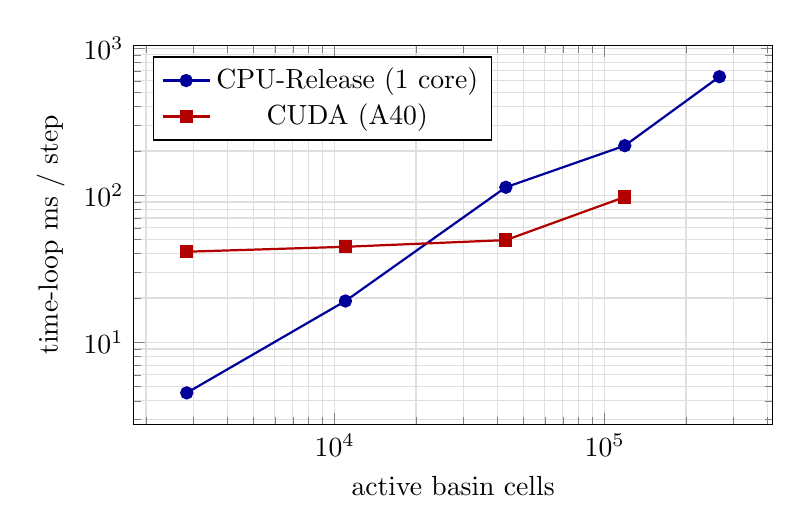
\begin{tikzpicture}
\begin{axis}[
    width=0.8\linewidth, height=6.4cm,
    xmode=log, ymode=log,
    xlabel={active basin cells}, ylabel={time-loop ms / step},
    legend pos=north west, grid=both, grid style={gray!25},
    ]
\addplot[thick,mark=*,color=blue!60!black]   coordinates {
    (2830,4.53) (10956,19.09) (43029,113.32) (118665,217.30) (266026,639.57) };
\addplot[thick,mark=square*,color=red!70!black] coordinates {
    (2830,41.30) (10956,44.61) (43029,49.54) (118665,97.31) };
\legend{CPU-Release (1 core), CUDA (A40)}
\end{axis}
\end{tikzpicture}
\caption{Per-step cost vs.\ problem size. The CPU scales roughly linearly with
the number of cells; the GPU is nearly flat until $\sim\!10^{5}$ cells
(launch/-sync bound), giving the crossover near $3\text{--}4\times10^{4}$ cells.}
\end{figure}

\paragraph{GPU warm-up.} The first CG solve pays a one-off cost (cuSPARSE /
cuBLAS descriptor creation, IC0 analysis, module load). From the \SI{50}{m}
runs, 5 steps $=\SI{2.96}{s}$ vs.\ 100 steps $=\SI{4.46}{s}$, i.e.\
$\approx\SI{8.9}{ms}$ per inner iteration in steady state plus
$\approx\SI{2.85}{s}$ fixed. Over a full \texttt{max\_Days} run (tens of
thousands of steps) this is negligible; the \SI{50}{m} loop then approaches
CPU $\SI{10.4}{ms}$ / GPU $\SI{8.9}{ms}$ per iteration ($\approx1.2\times$),
while at $15\text{--}25$~m the loop is already $2.2\text{--}2.3\times$ with the
warm-up still charged to only 100 steps.

\section{Known issues and next steps}
\label{sec:issues}

\begin{enumerate}\setlength\itemsep{3pt}
\item \textbf{\SI{10}{m} resolution ($2.7\times10^{5}$ cells) aborts} on the
      first step:
      \texttt{cuSPARSE API failed at line 1122 ... kernel launch failure (6)}
      in the PCG solve. The A40 is headless, so this is not a display-watchdog
      timeout --- most likely an out-of-bounds index in an assembly or stencil
      kernel that only manifests at this grid geometry, surfacing at the next
      cuSPARSE call. Next: \texttt{compute-sanitizer --tool memcheck} with
      \texttt{-steps 1 -scale 2}.
\item \textbf{No isolated unit tests.} Add per-wrapper tests that upload a small
      fixed field, run the kernel, and diff against the CPU function on the same
      data (bit-for-bit with \texttt{--fmad=false}, else a tolerance).
\item \textbf{No per-kernel timing.} Wrap each wrapper in an NVTX range /
      \texttt{cudaEvent} pair to get the breakdown (expected hot spots: CG
      solve, \texttt{buildMatrix}, interface kernels).
\item \textbf{Sediment / snow / gravitational kernels not numerically
      validated} --- need a snowmelt + rain-on-sediment event.
\item \textbf{CMake cache (resolved).} \texttt{build-cuda/CMakeCache.txt} had a
      stale \texttt{CMAKE\_CUDA\_ARCHITECTURES=75}; the compile line was in fact
      already \texttt{arch=compute\_86,code=[compute\_86,sm\_86]} (from the
      \texttt{set()} in \texttt{CMakeLists.txt}), so the binary was native for
      the A40, but the cache entry was reconfigured to \texttt{86} to remove the
      inconsistency.
\item \textbf{\texttt{--use\_fast\_math}:} keep for production speed, but build
      a \texttt{--fmad=false} variant for the validation runs so CPU/GPU can be
      compared at tighter tolerance.
\end{enumerate}

\section{Reproduction}

\begin{Verbatim}[fontsize=\small,xleftmargin=1em,breaklines=true,breakanywhere=true]
# builds
cmake -S DeterministicProgram -B build      -DENABLE_CUDA=OFF -DCMAKE_BUILD_TYPE=Release
cmake -S DeterministicProgram -B build-cuda  -DENABLE_CUDA=ON  -DCMAKE_BUILD_TYPE=Release
cmake --build build --parallel ; cmake --build build-cuda --parallel

# one benchmarked run, CUDA build, stop after 100 accepted steps
#   (STEPS -> "-steps N"; BUILD_DIR picks the build tree)
cd run
STEPS=100 BUILD_DIR=build-cuda ./submission_cuda.sh 5      # res 5 -> 25 m
#   -> ../Outputs/sim_ev_r5/run/out.1  contains the [BENCH] / [FP] lines

# full size sweep, both backends, results in ../Outputs/bench_sweep/summary.txt
STEPS=100 ./benchmark_sweep.sh 20 10 5 3
\end{Verbatim}

\end{document}
